\chapter{IMPLEMENTATION}

    All the encoding methods discussed throughout this thesis were implemented using Horovod \cite{alex2018horovod}; a tool that performs data parallelism for the distributed training of deep neural networks.
    Horovod provides support for various existing deep learning frameworks such as Tensorflow, PyTorch or MaxNet.
    
    Remember that, in most modern deep learning frameworks neural networks are represented as dataflow graphs whose nodes are commonly called operators and indicate the computations that need to take place.
    Horovod works by extending those graphs with an additional set of operators. Those perform the MPI communication for the gradients exchange between the workers, as well as the aggregation of them.
    Of course, it provides a different implementation for every such operator depending on the underlying deep learning framework.
    Horovod is also responsible for replicating the model in all the different workers, splitting the dataset into partitions, assigning these partitions to the workers and managing their overall synchronization in general. 
    
    \begin{figure}[h]
    \centering
    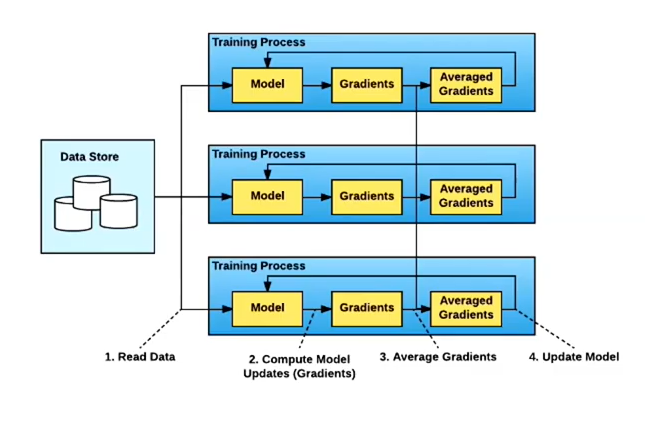
\includegraphics[width=0.7\textwidth]{thesis/figures/DataParallelism.png}
    \caption{Data Parallelism}
    \end{figure}

    This tool provides an ideal framework for embedding our own compression and decompression operators inside the computational graphs.
    Commonly, every operator that performs an MPI communication is "sandwiched" between two operators we call "Compressor" and "Decompressor", respectively, so that each gradient is encoded before it is sent off to the network and decoded after it is received by the worker.

    The deep learning framework we decided to use for this research work is TensorFlow and the various compression and decompression operations we experimented with were implemented either by using existing TensorFlow primitive operators or by creating our own custom operators in C++.

    More specifically, the bloom filter compressor and decompressor were implemented as custom TensorFlow operators.
    The algorithms needed for creating the bloom filters, posing queries and manipulating bits are highly procedural in nature and require a lot of side effects. Thus, dataflow was not the appropriate programming paradigm for encoding these kind of computations.
    

    % \begin{figure}[h]
    % \centering
    % 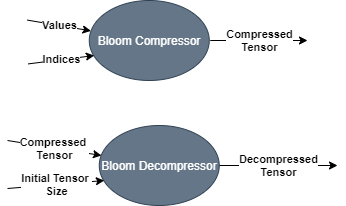
\includegraphics[width=0.7\textwidth]{thesis/figures/bloom-operators.png}
    % \caption{Bloom Filter Compressor/Decompressor}
    % \end{figure}
